%----------------------------------------------------------------------------------------
%	PACKAGES AND OTHER DOCUMENT CONFIGURATIONS
%----------------------------------------------------------------------------------------

\documentclass[12pt]{article}

\usepackage[utf8]{inputenc}
\usepackage[T1]{fontenc}
\usepackage{lmodern}
\usepackage{parselines}
\usepackage[portuguese]{babel}
\usepackage{graphicx}
\usepackage[document]{ragged2e}
\usepackage{listings}
\usepackage{xcolor}
\usepackage{geometry}
\geometry{
	a4paper,
	total={170mm,257mm},
	left=30mm,
	right=30mm,
	top=30mm,
	bottom=30mm,
}
\usepackage{amsmath}
\usepackage{hyperref}
\usepackage{url}
\usepackage{float}
\usepackage{tabularx}
\usepackage{booktabs}
\usepackage{indentfirst}
\usepackage{colortbl}
\usepackage{caption} 
\usepackage{enumitem}
\usepackage{hyperref}
\usepackage{listings}
\captionsetup[table]{skip=10pt}

\graphicspath{ {images/} }

\colorlet{punct}{red!60!black}
\definecolor{background}{HTML}{EEEEEE}
\definecolor{delim}{RGB}{20,105,176}
\colorlet{numb}{magenta!60!black}


\lstdefinelanguage{json}{
    basicstyle=\normalfont\ttfamily,
    numbers=left,
    numberstyle=\scriptsize,
    stepnumber=1,
    numbersep=8pt,
    showstringspaces=false,
    breaklines=true,
    frame=lines,
    backgroundcolor=\color{background},
    literate=
     *{0}{{{\color{numb}0}}}{1}
      {1}{{{\color{numb}1}}}{1}
      {2}{{{\color{numb}2}}}{1}
      {3}{{{\color{numb}3}}}{1}
      {4}{{{\color{numb}4}}}{1}
      {5}{{{\color{numb}5}}}{1}
      {6}{{{\color{numb}6}}}{1}
      {7}{{{\color{numb}7}}}{1}
      {8}{{{\color{numb}8}}}{1}
      {9}{{{\color{numb}9}}}{1}
      {:}{{{\color{punct}{:}}}}{1}
      {,}{{{\color{punct}{,}}}}{1}
      {\{}{{{\color{delim}{\{}}}}{1}
      {\}}{{{\color{delim}{\}}}}}{1}
      {[}{{{\color{delim}{[}}}}{1}
      {]}{{{\color{delim}{]}}}}{1},
}

\definecolor{dkgreen}{rgb}{0,0.6,0}
\definecolor{gray}{rgb}{0.5,0.5,0.5}
\definecolor{mauve}{rgb}{0.58,0,0.82}

\lstset{frame=tb,
  language=Java,
  aboveskip=3mm,
  belowskip=3mm,
  showstringspaces=false,
  columns=flexible,
  basicstyle={\small\ttfamily},
  numbers=none,
  numberstyle=\tiny\color{gray},
  keywordstyle=\color{blue},
  commentstyle=\color{dkgreen},
  stringstyle=\color{mauve},
  breaklines=true,
  breakatwhitespace=true,
  tabsize=3
}

\hypersetup{
  colorlinks, linkcolor=black
}

\begin{document}

\begin{titlepage}

\newcommand{\HRule}{\rule{\linewidth}{1mm}} % Defines a new command for the horizontal lines, change thickness here

\center % Center everything on the page
 
%----------------------------------------------------------------------------------------
%	HEADING SECTIONS
%----------------------------------------------------------------------------------------


\includegraphics{feup.jpg}

\textsc{\large Agentes e Inteligência Artificial Distribuída}\\[0.8cm] % Major heading such as course name
\textsc{\large 4º ano do Mestrado Integrado em Engenharia Informática e Computação}\\[0.8cm] % Minor heading such as course title

%----------------------------------------------------------------------------------------
%	TITLE SECTION
%----------------------------------------------------------------------------------------

\HRule \\[1.2cm]
{ \huge \bfseries \textit{Simulação de Evacuação com Agentes}}\\[0.6cm] % Title of your document
{ \large \bfseries Relatório de Implementação} \\[0.6cm]
\HRule \\[2cm]
 
%----------------------------------------------------------------------------------------
%	AUTHOR SECTION
%----------------------------------------------------------------------------------------


% If you don't want a supervisor, uncomment the two lines below and remove the section above
\Large \emph{Estudantes:}\\[0.5cm] \normalsize
Gil \textsc{Domingues}\\[0.1cm]  
- up201304646@fe.up.pt\\[0.1cm]
Pedro \textsc{Pontes}\\[0.1cm]
- up201305367@fe.up.pt\\[2cm] 

%----------------------------------------------------------------------------------------
%	DATE SECTION
%----------------------------------------------------------------------------------------

{\large \today}\\[0cm] % Date, change the \today to a set date if you want to be precise

%----------------------------------------------------------------------------------------
%	TABLE OF CONTENTS & LISTS OF FIGURES AND TABLES
%----------------------------------------------------------------------------------------

\clearpage 

\tableofcontents

\clearpage 
%----------------------------------------------------------------------------------------
%	INTRODUÇÃO
%----------------------------------------------------------------------------------------
\justify\normalsize

\section{Introdução} 

Uma evacuação implica mover pessoas de um dado local devido à ocorrência de uma situação de (potencial) catástrofe. Exemplos incluem a evacuação de um edifício em chamas ou de uma localidade, antes, durante ou após um desastre natural, como uma cheia ou terramoto. 

Evacuar grandes multidões é um desafio, independentemente das circunstâncias. Tipicamente, de uma evacuação de emergência resultam feridos - ou mesmo mortes -, devido ao caos e pânico que se geram.

Com o aumento da frequência de situações que implicam a evacuação de um elevado número de pessoas num curto espaço de tempo, existe uma consciência acrescida da importância do planeamento dessas situações.

Com efeito, a gestão e organização de multidões em situações de emergência tornou-se uma importante área de estudo ao longo dos últimos anos e desempenha, hoje, um papel importante no planeamento de um edifício ou área.

Dados os desafios - quer de ordem prática, quer de ordem financeira - que a realização de simulacros coloca, é cada vez mais comum o uso de técnicas de simulação para estudar estas situações. De facto, existem já diversos tipos de sistemas, como as simulações baseadas na dinâmica de fluídos, as simulações baseadas em autómatos e as simulações baseadas em agentes.

%----------------------------------------------------------------------------------------
%	CONTEXTO 
%----------------------------------------------------------------------------------------

\section{Contexto}

\subsection{Cenário}

Ocorreu um incêndio, uma inundação, a libertação de um gás nocivo, um qualquer acidente que obriga à evacuação daqueles presentes num dado local. O local possui múltiplas saídas de emergência e também obstáculos. Os indivíduos encontram-se distribuídos pelo local, ocupados nas suas tarefas usuais. Aquando da deteção do acidente, todos os indivíduos procuram atingir uma das saídas de emergência, o mais rapidamente possível.

Alguns agentes poderão ser altruístas, no sentido de ajudarem acidentados a deslocarem-se até à saída, outros poderão simplesmente querer «salvar a pele», exibindo um comportamento mais egoísta. Alguns poderão conhecer bem o local e, como tal, chegar rapidamente à saída, outros demorarão mais ou mesmo perder-se, tendo que pedir ajuda. 


\subsection{Objetivos}

Realizado no âmbito da unidade curricular de Agentes e Inteligência Artificial Distribuída, com este projeto pretende desenvolver-se um programa que permita simular a interação de agentes confinados a um espaço concreto e limitado perante a necessidade de evacuar esse espaço, podendo o utilizador definir diferentes cenários, especificando, por um lado, o tipo, número e localização dos agentes a evacuar e, por outro, o número e localização de saídas de emergência e obstáculos. 

%----------------------------------------------------------------------------------------
%	ESPECIFICAÇÃO
%----------------------------------------------------------------------------------------

\newpage
\section{Especificação}
\subsection{Agentes}

Podem distinguir-se dimensões distintas no comportamento exibido durante uma evacuação: por um lado, o espaço a evacuar e a sua configuração, e, por outro lado, as características psicológicas e sociais que afetam a resposta dos que participam na evacuação.

Assume-se que, em situações de emergência, os indivíduos entram em pânico e ficam, por isso, propensos a tomar decisões irracionais. Mais ainda, as pessoas tentam mover-se tão depressa quanto possível, devendo evitar obstáculos.

Deste modo, tem-se que os agentes implementados são autónomos, proativos e reativos e são caracterizados por diversos atributos, conforme definido na Tabela 1.

\setlength{\tabcolsep}{20pt}
\renewcommand{\arraystretch}{1.3}
\begin{table}[H]
	\centering
	\label{agent-attributes}
	\caption{Atributos dos agentes implementados, que condicionam os seus comportamentos.}
	\begin{tabular}{@{}lll@{}}
		\toprule
		\rowcolor[HTML]{FFFFFF} 
	\textbf{Atributos}           & \textbf{Tipo}  & \textbf{Descrição}                                                                                                                                   \\ \toprule
		\rowcolor[HTML]{FFFFFF} 
		idade                & int   & {[}5, 65{]}                                                                                                                                 \\ \midrule
		\rowcolor[HTML]{FFFFFF} 
		género               & Enum   & \{Masculino, Feminino\} \\ \midrule
		\rowcolor[HTML]{FFFFFF} 
		conhecimento da área & int & \begin{tabular}[c]{@{}l@{}}{[}0, 100{]} \\probabilidade de seguir o melhor\\ caminho até uma saída \\\end{tabular}                                                                                                                                     \\ \midrule
		\rowcolor[HTML]{FFFFFF} 
		independência        & int   & \begin{tabular}[c]{@{}l@{}}{[}0, 100{]} \\probabilidade de seguir (ou não) outros\\\end{tabular}  \\ \midrule
		\rowcolor[HTML]{FFFFFF} 
		altruísmo   & int & \begin{tabular}[c]{@{}l@{}}{[}0, 100{]} \\probabilidade para ajudar outros\\\end{tabular}    \\ \midrule                                                 
		\rowcolor[HTML]{FFFFFF} 
		mobilidade   & int & \begin{tabular}[c]{@{}l@{}}{[}0, 100{]}\\ condiciona a probabilidade de se mover\\num dado instante \end{tabular} \\
		\midrule
		\rowcolor[HTML]{FFFFFF} 
		estado de pânico     & int & \begin{tabular}[c]{@{}l@{}}{[}0,100{]}\\ afeta o discernimento da pessoa\end{tabular}\\ \midrule
		\rowcolor[HTML]{FFFFFF} 
		paciência     & int & \begin{tabular}[c]{@{}l@{}}{[}0,100{]}\\determina a probabilidade de reagir de\\ intempestivamente\end{tabular}                                                   \\ \midrule
	\end{tabular}

\end{table}
\newpage

Em função dos atributos de independência e de conhecimento da área, considerou-se a categorização dos agentes em quatro estereótipos, conforme descrito na Tabela 2.

\setlength{\tabcolsep}{20pt}
\renewcommand{\arraystretch}{1.3}
\begin{table}[H]
	\centering
	\label{agent-types}
	\caption{Diferentes tipos de agente, de acordo com os valore possíveis para os atributos considerados.}
	\begin{tabular}{@{}lll@{}}
		\toprule
		\rowcolor[HTML]{FFFFFF} 
		\textbf{Tipo}  & 
		\begin{tabular}{@{}lll@{}}
			\textbf{Atributos} \\
			independence & areaKnowledge\end{tabular}\\ \toprule
		\rowcolor[HTML]{FFFFFF} 
		IndependentKnowledgeable &
		\begin{tabular}{@{}lll@{}}
			 [50, 100] & \hspace{.8cm} [50, 100] \end{tabular}\\ \midrule 
		 \rowcolor[HTML]{FFFFFF} 
		 IndependentUnknowledgeable &
		 \begin{tabular}{@{}lll@{}}
		 	[50, 100] & \hspace{.8cm} [0, 50] \end{tabular}\\ \midrule 
		 DependentKnowledgeable &
		 \begin{tabular}{@{}lll@{}}
		 	[0, 50] & \hspace{1.2cm} [50, 100] \end{tabular}\\ \midrule 
		DependentUnknowledgeable &
 		\begin{tabular}{@{}lll@{}}
 			[0, 50] & \hspace{1.2cm} [0, 50] \end{tabular}\\ \midrule 
	\end{tabular}
\end{table}

Esta classificação permitiu a definição, ao nível de interface, de diferentes representações para os vários tipos de agente, permitindo estabelecer visualmente a relação entre o tipo de agente e os seus comportamentos.

\setlength{\tabcolsep}{20pt}
\renewcommand{\arraystretch}{1.3}
\begin{table}[H]
	\centering
	\label{agent-behaviours}
	\caption{Comportamentos dos agentes.}
	\begin{tabular}{@{}lll@{}}
		\toprule
		\rowcolor[HTML]{FFFFFF} 
		\textbf{Comportamento}  & \textbf{Descrição}                                                                                                                                   \\ \toprule
		\rowcolor[HTML]{FFFFFF} 
		\begin{tabular}[c]{@{}l@{}}Processo de\\Evacuação\end{tabular} & \begin{tabular}[c]{@{}l@{}}A cada momento um agente deve usar o seu\\conhecimento da área e mover-se em direção à saída.\end{tabular}  \\ \midrule 
		\rowcolor[HTML]{FFFFFF} 
	    \begin{tabular}[c]{@{}l@{}}Mecanismo de\\Pânico\end{tabular} & \begin{tabular}[c]{@{}l@{}}A cada momento um agente atualiza o seu estado\\ de pânico de acordo com a sua condição e o\\ambiente envolvente.\end{tabular}  \\ \midrule 
	    \rowcolor[HTML]{FFFFFF} 
	    \begin{tabular}[c]{@{}l@{}}Sentido de\\Altruísmo\end{tabular} & \begin{tabular}[c]{@{}l@{}}A cada momento um agente monitoriza o ambiente\\ envolvente e decide responder ou ignorar pedidos de\\ ajuda de outros agentes.\end{tabular}  \\ \midrule 
	    \rowcolor[HTML]{FFFFFF} 
	    \begin{tabular}[c]{@{}l@{}}Pedido de\\Direções\end{tabular} & \begin{tabular}[c]{@{}l@{}}Um agente toma, por ser pouco independente ou ter\\pouco conhecimento da área, pede direções a agentes\\ na sua proximidade.\end{tabular}  \\ \midrule 
	    \rowcolor[HTML]{FFFFFF} 
	    \begin{tabular}[c]{@{}l@{}}Pedido de\\Ajuda\end{tabular} & \begin{tabular}[c]{@{}l@{}}Um agente incapaz de se mover de forma autónoma\\ pede ajuda aos agentes na sua proximidade.\end{tabular}  \\ \midrule 
		                                                       
	\end{tabular}
	
\end{table}

\subsection{Interações}

A comunicação entre agentes foi implementada recorrendo a mensagens \textit{JADE}, obedecendo aos protocolos \textit{FIPA}. 

Dado que todos os agentes se encontram, a cada momento, numa dada posição de um espaço, cada agente pode tomar conhecimento daqueles que o rodeiam, sendo possível obter os seus \textit{AID}’s usando a noção de proximidade.\newline

\renewcommand{\lstlistingname}{Excerto}

\begin{lstlisting}[caption= Código \textit{Java}\, ilustrando a possibilidade de uma pessoa poder descobrir outras.]
// find people in the surrounding area
ArrayList<AID> peopleNear = environment.findNear(myAgent);
if(peopleNear.isEmpty()) {
	return;
}
\end{lstlisting}

\paragraph{}

Os vários agentes assumem uma atitude mais ou menos cooperativa, em função dos atributos altruísmo e independência, e partilham um objetivo comum: chegar a uma saída.
\newline

Com vista a simular de forma algo fidedigna as condições de uma evacuação de emergência, foram implementadas as seguintes interações entre agentes:

\begin{itemize}

\item Terror;

Um agente cujo nível de pânico sobe acima de um certo nível envia uma mensagem \textit{PROPAGATE} para agentes na proximidade.

Aqueles que recebem esta mensagem, podem, ou não, propagar a mensagem e aumentam o seu estado de pânico - variação que depende de diversos fatores: assumiu-se que as pessoas mais independentes são menos influenciáveis pelos gritos dos outros enquanto os mais jovens ou mais idosos são mais impressionáveis.\newline



\begin{figure}[H]
	\centering
	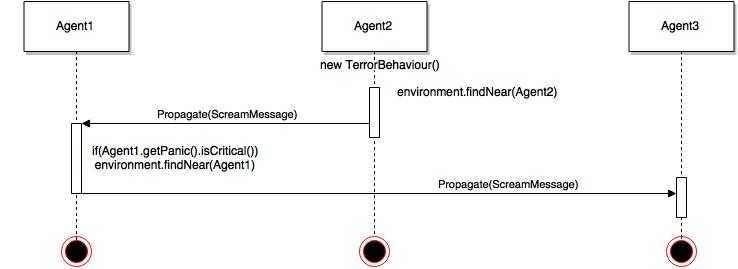
\includegraphics[scale=0.5]{terror-behaviour.jpg}
	\caption{Diagrama de sequência exemplificando uma interação do tipo Terror.}
	\label{uml}
\end{figure}

\item Orientação.

Duas pessoas podem partilhar conhecimento sobre a área, mediante um pedido nesse sentido. Um agente que tenha pouco conhecimento da área pode enviar a um agente ao seu redor uma mensagem \textit{CFP}, a que esse agente responde com uma dada probabilidade - dependente do valor do atributo altruísmo. A resposta consiste numa mensagem \textit{INFORM}, com o valor do seu conhecimento da área, \textit{conhecimento1}. Por forma a simular a aquisição de informação, o agente que fez o pedido atualizará o seu nível de conhecimento da área, \textit{conhecimento2}, de acordo com:

\[	conhecimento2 = max(conhecimento2, conhecimento1 * 0.80) \]

\begin{figure}[H]
	\centering
	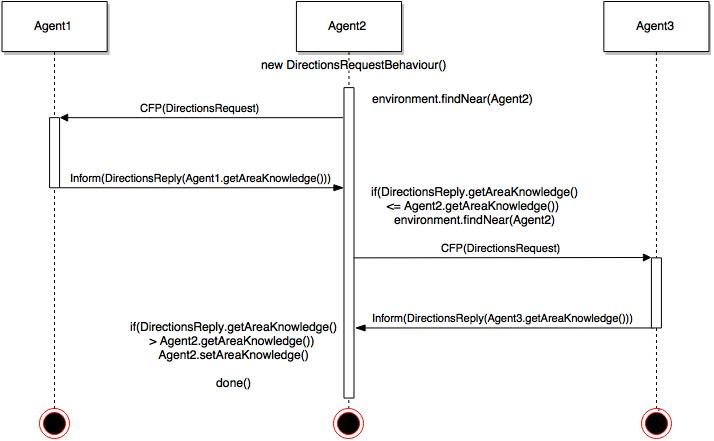
\includegraphics[scale=0.5]{directions-behaviour.jpg}
	\caption{Diagrama de sequência exemplificando uma interação do tipo Orientação.}
	\label{uml}
\end{figure}



\item Ajuda;

Um agente pode pedir ajuda, enviando uma mensagem \textit{CFP} para agentes ao seu redor. Os agentes na disposição de ajudar podem oferecer a sua ajuda, enviando uma mensagem \textit{PROPOSAL}, com o valor da sua mobilidade, \textit{mobilidade1}.

O autor do pedido de ajuda aceita uma oferta, respondendo com uma mensagem \textit{ACCEPT\_PROPOSAL}, com o valor da sua mobilidade, \textit{mobilidade2}. O agente que ofereceu ajuda passa a guiar o outro até à saída, sendo a mobilidade de cada um dada por:

\[	mobilidade1 = mobilidade2 = \frac{mobilidade1 + moblidade2}{2} \]

\begin{figure}[H]
	\centering
	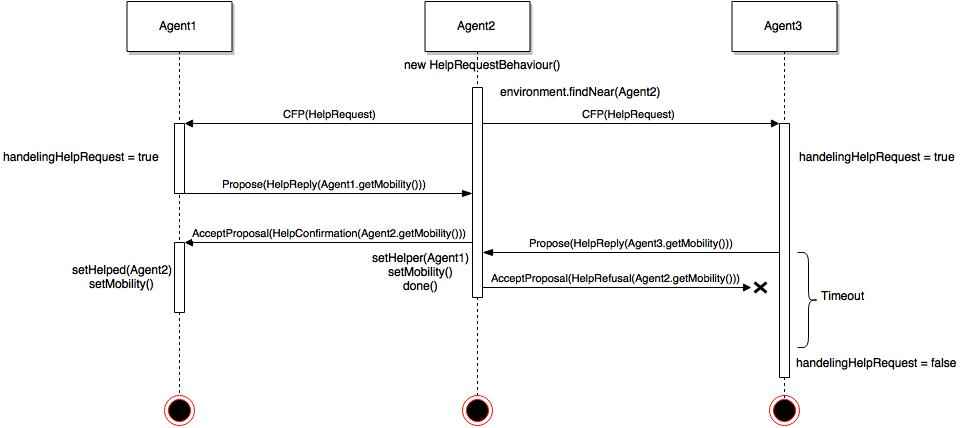
\includegraphics[scale=0.4]{help-behaviour.jpg}
	\caption{Diagrama de sequência exemplificando uma interação do tipo Ajuda.}
	\label{uml}
\end{figure}

\end{itemize}

Como pode constatar-se, estes protocolos são relativamente simples. De referir, ainda, que as interações Ajudar e Orientar são efetuadas de acordo com o modelo de Rede Contratual, sendo que, no caso, o papel de gestor cabe ao agente que faz o pedido inicial. 


%----------------------------------------------------------------------------------------
%	DESENVOLVIMENTO
%----------------------------------------------------------------------------------------

\newpage
\section{Desenvolvimento}
\subsection{Faseamento}
A implementação do projeto executou-se em diferentes etapas:
\begin{enumerate}
	\item Especificação e planeamento (23 de outubro a 1 de novembro);
	\item Implementação de:
	 \begin{enumerate} 
	 	\item Agente (25 de outubro a 5 de novembro);
	 	\item Espaço (5 de novembro a 25 de novembro);
	 	
	 	Teste e análise do comportamento de um agente num espaço.
		\item Interação entre agentes (5 de novembro a 5 de dezembro);
		
		Teste e análise do comportamento de vários agentes num espaço. 
	\end{enumerate}
	\item Exploração de diferentes cenários e recolha e avaliação de métricas (1 de dezembro a 10 de dezembro).
\end{enumerate}

\subsection{Ambiente de Desenvolvimento e Ferramentas}
O desenvolvimento decorreu em ambiente Windows 10 e usando a versão Neon do \textit{IDE Eclipse}, tendo-se feito uso das ferramentas \textit{JADE}, \textit{Repast Simphony} e \textit{SAJaS}.
\newline

\textbf{\textit{JADE}:} Definição de agentes.

\textbf{\textit{Repast Simphony}:} Simulação multiagente.

\textbf{\textit{SAJaS}:} Integração de agentes \textit{JADE} com \textit{Repast}.
\newline

O \textit{Repast} é uma \textit{framework open-source} que permite criar, analisar e experimentar com mundos artificiais populados por agentes que interagem de forma não trivial.

Concretamente, irá utilizar-se a sua mais recente versão - \textit{Repast Simphony}, que permite programar em \textit{Java} a estrutura espacial, a estrutura lógica e os comportamentos dos agentes.

Tendo sido amplamente utilizado em aplicações de simulação, considera-se de particular utilidade, por um lado, o foco em modelar o comportamento social e, por outro, a recolha de métricas associadas às simulações realizadas. Por último, tem-se a vantagem de poder acompanhar, de forma visual, o decorrer da simulação.

Adicionalmente, irá utilizar-se a \textit{API SAJaS}, que possibilita a integração de agentes \textit{JADE} com \textit{Repast}, permitindo definir os comportamentos de agentes e fazer uso das capacidades de comunicação entre agentes, visando simular as interações expectáveis num cenário de evacuação.

\subsection{Estrutura}

Estrutura da aplicação, módulos, diagrama de classes...
(incluir UML)

\begin{figure}[H]
	\centering
	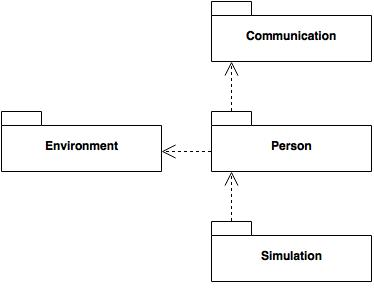
\includegraphics[scale=0.5]{packages.jpg}
	\caption{Diagrama de pacotes, ilustrativo da estrutura lógica do projeto.}
	\label{uml}
\end{figure}

\begin{figure}[H]
	\centering
	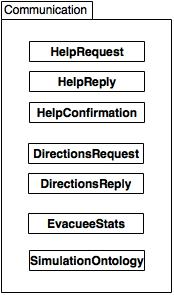
\includegraphics[scale=0.5]{communication.jpg}
	\caption{Classes do pacote \textit{Communication}.}
	\label{uml}
\end{figure}

\subsection{Detalhes}
\subsubsection{Agentes}
Detalhes de implementação sobre o agentes

\subsubsection{Ambiente}
Detalhes de implementação sobre o ambiente/espaço.

\newpage
\section{Experimentação}

Ao longo do processo de desenvolvimento foram levadas a cabo múltiplas experiências, com vista a testar a implementação dos Agentes.
\begin{itemize}
	
%----------------------------------------------------------------------------------------
%	EXP begin
%----------------------------------------------------------------------------------------
	
\item \textbf{Evacuação simples}

\textbf{Objetivo:} 
                                                                                                                                  	Testar se um agente é capaz de atingir a saída.
	
Esta experiência consistiu na colocação, num espaço pré-definido, de um agente de um determinado tipo, tendo-se analisado o seu comportamento e medido o tempo que decorreu até que chegasse à saída.
	
\setlength{\tabcolsep}{20pt}
\renewcommand{\arraystretch}{1.3}
\begin{table}[H]
	\centering
	\begin{tabular}{@{}lll@{}}
		\toprule
		\rowcolor[HTML]{FFFFFF} 
		\textbf{Tipo de agente}  & \textbf{Tempo de evacuação}                                                                                                                                   \\ \toprule
		\rowcolor[HTML]{FFFFFF} 
		IndependentKnowledgeable &
		????\\ \midrule 
		\rowcolor[HTML]{FFFFFF} 
		Independent &
		?????\\ \midrule 
		Knowledgeable &
		??????\\ \midrule 
		DependentUnknowledgeable &
		?????\\ \midrule 
	\end{tabular}
\end{table}
	
	Como esperado, observou-se que os agentes com maior conhecimento da área demoraram menos tempo a chega à saída.
	
	Dado que, nesta fase, se utilizou apenas um agente de cada tipo, o atributo independência não se reflete no desempenho do agente.
	
%----------------------------------------------------------------------------------------
%	EXP end
%----------------------------------------------------------------------------------------
	
\end{itemize}


Terminada a fase de desenvolvimento, foram avaliados diferentes cenários.
\begin{itemize}
	\item diferentes configurações para o local do acidente, variando o número e localização de saídas de emergência e obstáculos;
	\item diferentes combinações de agentes a evacuar, variando o seu tipo, número ou localização.
\end{itemize}

Deste modo, será possível observar-se como estas variações se refletem em métricas como o tempo médio e máximo de evacuação ou o número de feridos.

\newpage
\section{Conclusão}

Terminado o projeto, destaca-se a importância de ferramentas de simulação de evacuação, perante os desafios que a realização de simulacros coloca.

Consideram-se atingidos os objetivos definidos: desenvolver um programa que permita simular a interação de agentes confinados a um espaço concreto e limitado perante a necessidade de evacuar esse espaço.

Da análise dos resultados das experiências levadas a cabo
Do desenvolvimento do trabalho e aplicabilidade de SMA ao cenário proposto
Trabalho futuro



\section{Recursos}
\subsection{Bibliografia}
[1] Almeida, João; Rosseti, Rosaldo; Coelho, António: \textit{Crowd Simulation Modeling Applied to Emergency and Evacuation Simulations using Multi-Agent Systems}. 2011.

[2] FIPA: \textit{FIPA Specification}. Disponível online em \url{http://www.fipa.org/specs/fipa00037/SC00037J.pdf}. Consultado em novembro de 2016.

[3] Respast: \textit{Repast Simphony Documentation}. Disponível online em \url{http://repast.sourceforge.net/docs/api/repast_simphony/index.html}. Consultado em novembro de 2016.

[4] SAJaS: \textit{SAJaS Documentation}. Disponível online em \url{https://web.fe.up.pt/~hlc/doku.php?id=sajas}. Consultado em novembro de 2016.


\subsection{Software}
[1] \textit{Repast Simphony};

[2] \textit{JADE};

[3] \textit{SAJaS}.

[4] \textit{Eclipse};

\end{titlepage}
\end{document}